% Systematisk beskrivelse af konfigurations tabel.
\section{Konfigurationstabel}\label{konfigurationstabel}
En konfiguration af et system er en kombination af elementer, og en konfigurationstabel beskriver den konfiguration.
I \cref{tab:konfigurationsTabel} præsenteres konfigurationstabellen for projektet, og indholdet vil i de følgende sektion blive forklaret.

\begin{figure}
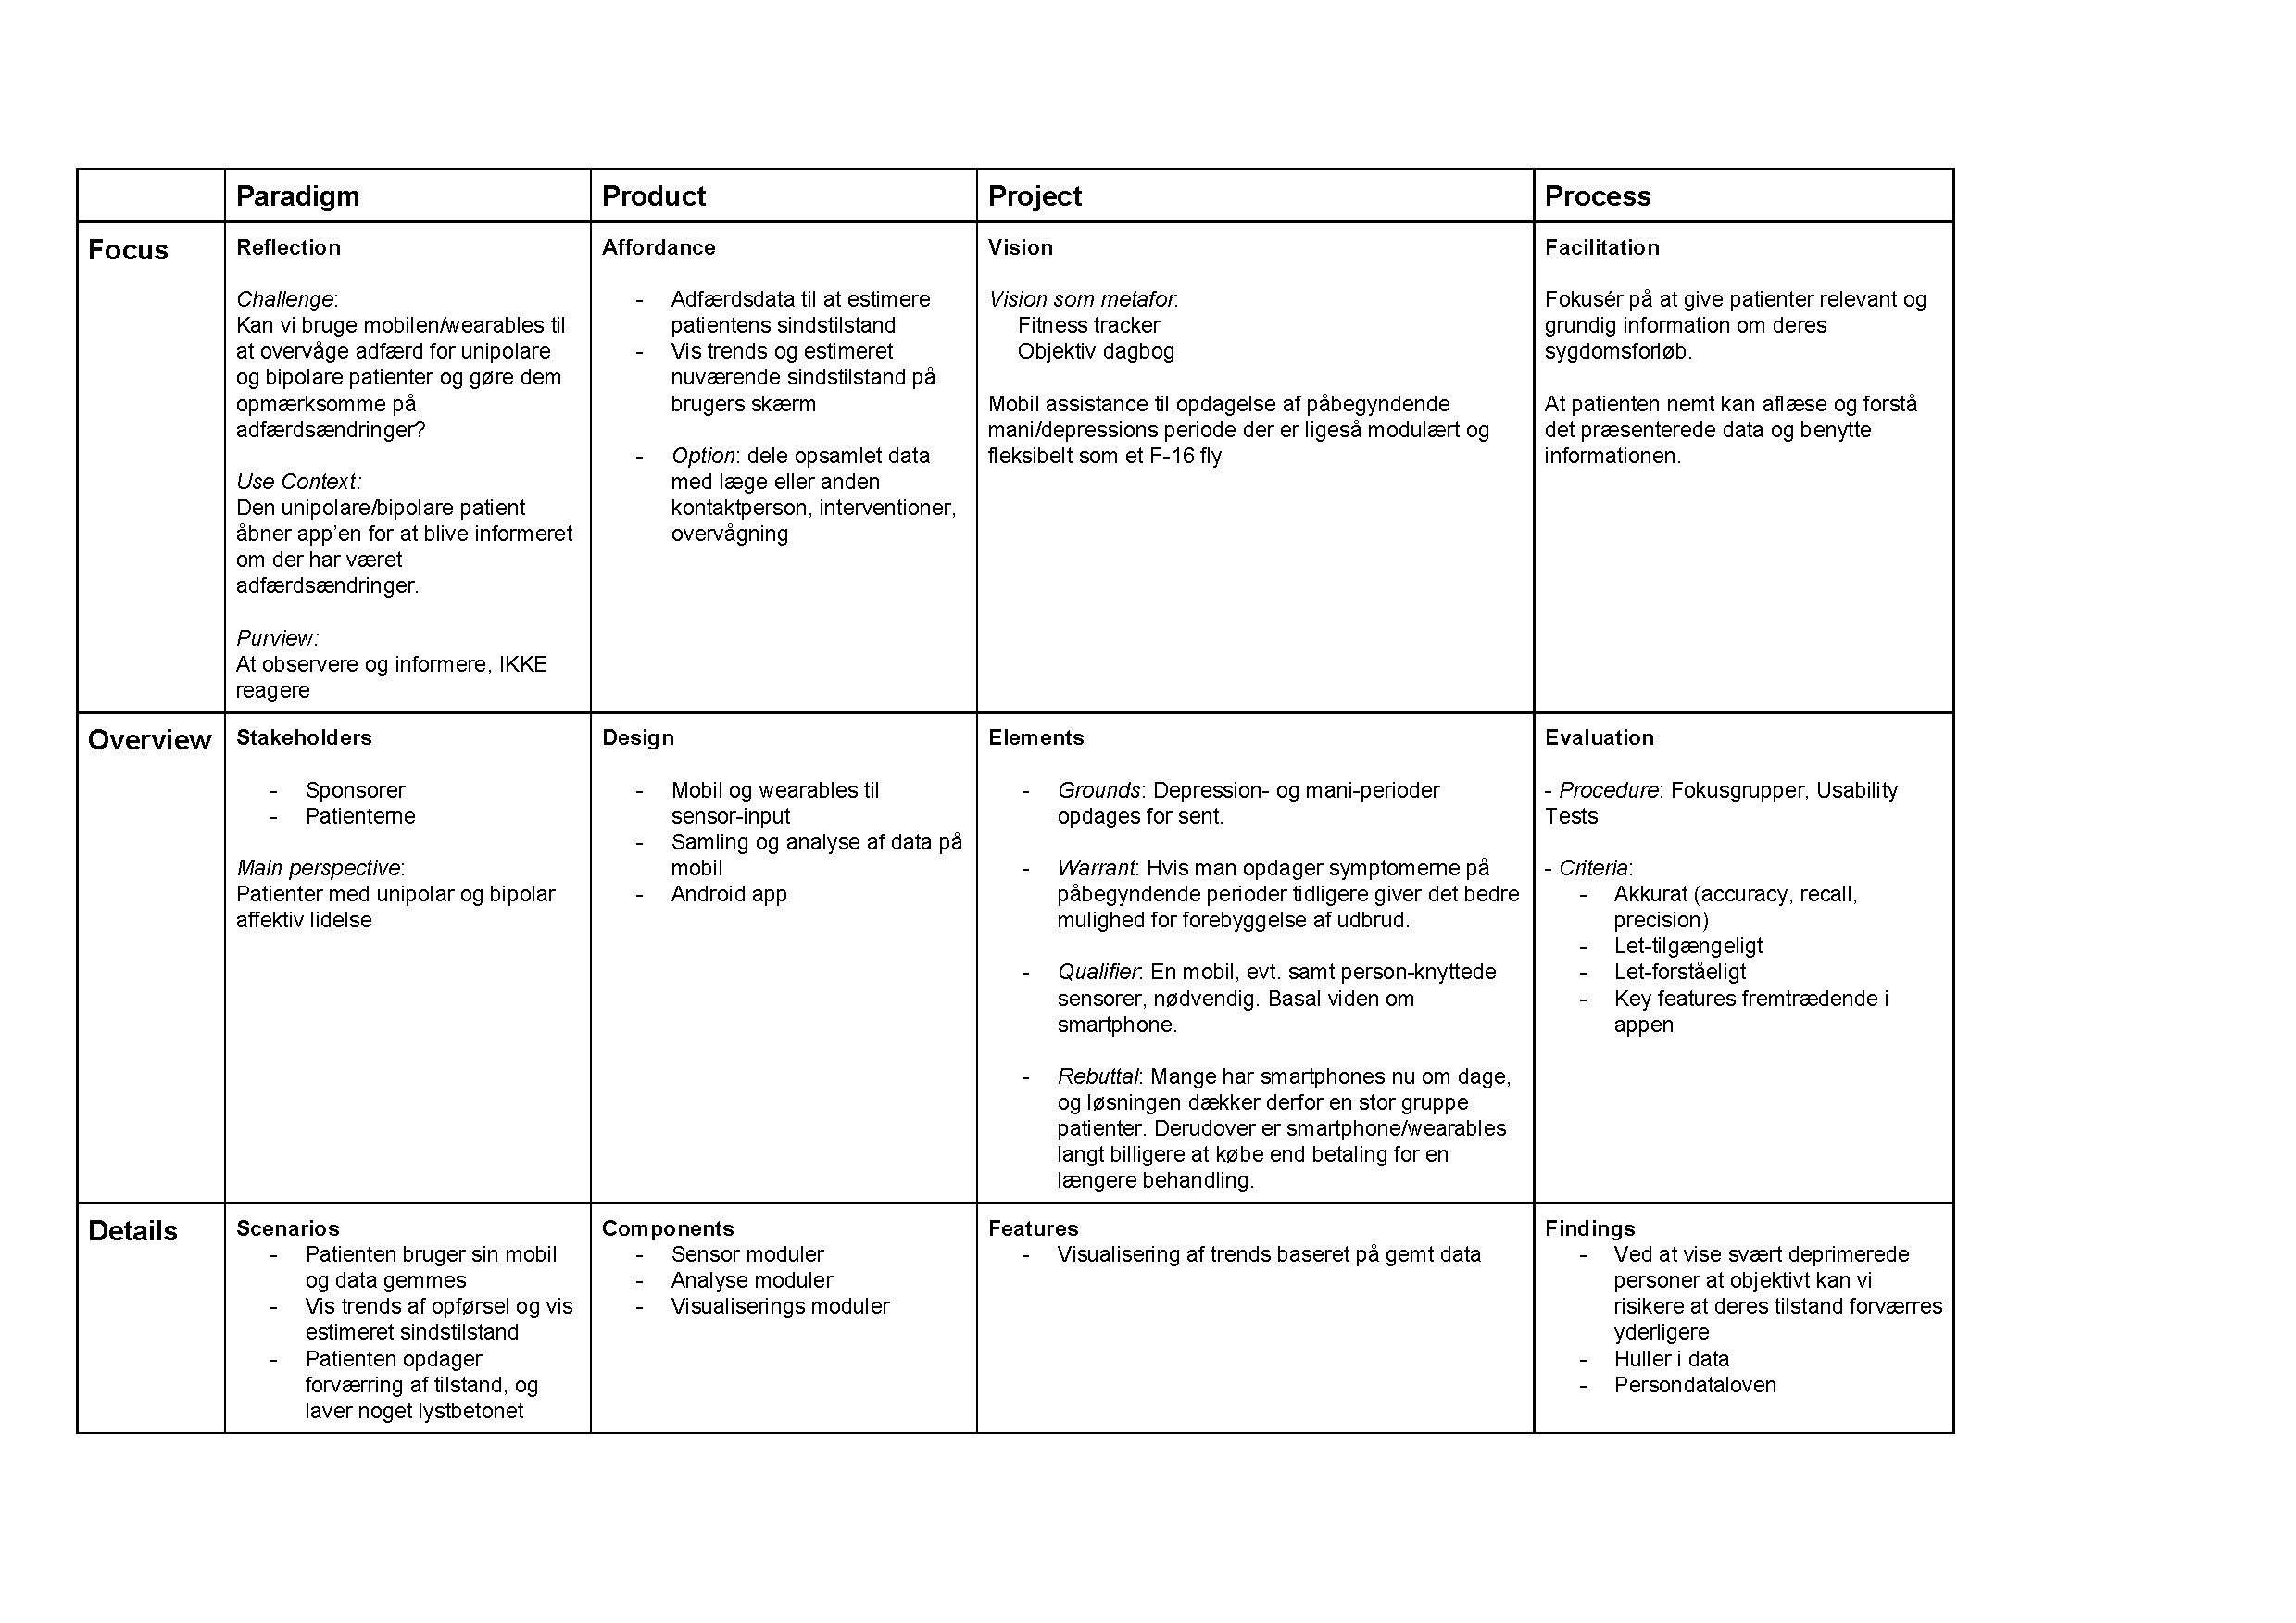
\includegraphics[scale = 0.65,trim = 1cm 3cm 6cm 2cm, angle = 90, clip]{KonfigurationTabel}
\caption{Konfigurations tabellen for systemet.}
\label{tab:konfigurationsTabel}
\end{figure}
